% !TEX program = xelatex
%% Requires compilation with XeLaTeX or LuaLaTeX
\documentclass[10pt,xcolor={table,dvipsnames},t]{beamer}
\usepackage{biblatex}
\usepackage{caption}
\setbeamertemplate{caption}[numbered]
\addbibresource{reference.bib}
\usepackage{hyperref}
\hypersetup{ 
pdfpagemode=FullScreen,  
colorlinks=true,linkcolor=blue}
\usepackage{enumerate}

\usepackage{listings}
\usepackage{xcolor}

\definecolor{codegreen}{rgb}{0,0.6,0}
\definecolor{codegray}{rgb}{0.5,0.5,0.5}
\definecolor{codepurple}{rgb}{0.58,0,0.82}
\definecolor{backcolour}{rgb}{0.95,0.95,0.92}

\lstdefinestyle{mystyle}{
    backgroundcolor=\color{backcolour},   
    commentstyle=\color{codegreen},
    keywordstyle=\color{magenta},
    numberstyle=\tiny\color{codegray},
    stringstyle=\color{codepurple},
    basicstyle=\ttfamily\footnotesize,
    breakatwhitespace=false,         
    breaklines=true,                 
    captionpos=b,                    
    keepspaces=true,                 
    numbers=left,                    
    numbersep=5pt,                  
    showspaces=false,                
    showstringspaces=false,
    showtabs=false,                  
    tabsize=2
}

\lstset{style=mystyle}

% Flow chart config
\usepackage{tikz}
\usetikzlibrary{calc,trees,positioning,arrows,fit,shapes,calc}
\usetikzlibrary{shapes.geometric, arrows}
\tikzstyle{startstop} = [rectangle, rounded corners, minimum width=3cm, minimum height=1cm,text centered, draw=black, fill=red!30]
\tikzstyle{io} = [trapezium, trapezium left angle=70, trapezium right angle=110, minimum width=3cm, minimum height=1cm, text centered, draw=black, fill=blue!30]
\tikzstyle{process} = [rectangle, minimum width=3cm, minimum height=1cm, text centered, draw=black, fill=orange!30]
\tikzstyle{decision} = [diamond, minimum width=3cm, minimum height=1cm, text centered, draw=black, fill=green!30]
\tikzstyle{arrow} = [thick,->,>=stealth]

\usetheme{UCBerkeley}

\title[Your Short Title]{STMC HKOI Training}
\subtitle{Lesson 4: Looping and Array}
\author{Tsai Yun Chen}
%\institute{}
\date{\today}

\begin{document}

\begin{frame}
  \titlepage
\end{frame}

% Uncomment these lines for an automatically generated outline.
%\begin{frame}{Outline}
%  \tableofcontents
%\end{frame}

\section{Class Goal}

\begin{frame}{Goal today}

\begin{itemize}
  \item Concept of loop
  \item \texttt{while} loop
  \item \texttt{for} loop using \texttt{range}
  \item The for loop \texttt{for}
  \item Basics \texttt{list} 
\end{itemize}

\end{frame}


\section{Concept of loop}
\begin{frame}{Loop: Repeat and repeat ....}
    \begin{itemize}
      \item Many times in programming we want the code to run repeatedly until certain conditions are met
      \vspace{2mm}
      \item For example:
      \begin{itemize}
        \item Recieving user input: User might input a wrong value. You would want to keep asking for an input until it's right
        \item Reading files: You want to keep reading lines until the end of file 
        \item Games: You want to keep the main code running until the game ends
        \item Searching: Sometimes you use computer to search for answers. You would want the computer to keep searching until the solution / close enough solution is reached
      \end{itemize}
    \end{itemize}
\end{frame}

\begin{frame}{Loop: Repeat and repeat ....}
  \begin{itemize}
    \item From the examples above, we see the a looping structure always consist of two parts:
    \begin{enumerate}
      \item The code inside the code that is looped over 
      \item A condition that is checked everytime the loop ran to decide whether the loop should continue
    \end{enumerate}
    \item  Example: 
    \begin{itemize}
      \item Recieving user input (code inside loop); Is the answer right (terminate condition)
      \item Reading files (code inside loop); Is the end of file reached (terminate condition)
      \item Main game code (code inside the loop); Is the game over (terminate condition)
      \item Searching for answers (code inside the loop); Is the solution found (terminate condition)
    \end{itemize}
  \end{itemize}
\end{frame}

\begin{frame}{Example: Print first $N$ positive integer}
\begin{itemize}
  \item Let's write a program that takes in an integer $N$ and print out all positive integers $i$ in range $1\leq i \leq N$
  \item For example:
  \begin{itemize}
    \item If we enter 1, \texttt{\{1\}} will be printed
    \item If we enter 4, \texttt{\{1,2,3,4\}} will be printed 
    \item and etc.
  \end{itemize}
\end{itemize}
\end{frame}

\begin{frame}[fragile]{Example: Print first $N$ positive integer}
  \begin{itemize}
    \item Some example input and output:
\begin{lstlisting}
  $./main       $./main       $./main 
  5             4             100
  1             1             1
  2             2             2
  3             3             .... /* too long won't list here*/
  4             4             99
  5                           100
\end{lstlisting}
  
  \item \textbf{Problem: How can we implement this in code?}
  \end{itemize}
\end{frame}

\begin{frame}{Flow chart}
  \begin{columns}
    \column{0.6\textwidth}
    \begin{itemize}
      \item Let's look at the flow chart
      \item Basically, we repeat certain blocks of code until a given condition (in this case $i\leq N$) is $false$
      \item This condition is called the \textbf{loop condition}
      \item Notice "Set i = i + 1" is crucial otherwise i will always be smaller than N. This will cause an \textbf{infinite loop}
    \end{itemize}
    \column{0.4\textwidth}
    \begin{figure}
      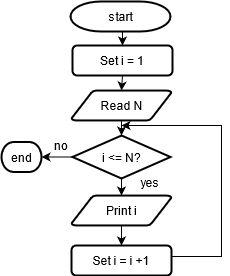
\includegraphics[width=0.9\textwidth]{img/print_first_n_flowchart.png}
    \end{figure}
  \end{columns}
\end{frame}

\section{While loop}
\begin{frame}[fragile]{\texttt{while} loop}
  \begin{itemize}
    \item In Python, we can implement that using \texttt{while} loop 
    \item Here is the syntax of \texttt{while} loop 
  \end{itemize}
\begin{lstlisting}[language=python]
while """loop condition""":
  # Remember to indent
  # This will keep looping as long as loop condition is True

# When loop condition is False, the loop will break 
# The code will continue to run from here
\end{lstlisting}
\end{frame}

\begin{frame}[fragile]{Example: Print first $N$ positive integer}
  \begin{itemize}
    \item This is how we write print first $N$ positive integer in python
  \end{itemize}
\begin{lstlisting}[language=python]
N = int(input('Enter N: '))
i = 1
while i <= N:
  print(i)   # Print i, remember to indent
  i = i + 1  # This is critical, otherwise infinite loop
print('End of story') # Just some useless print 
\end{lstlisting}
\end{frame}

% \begin{frame}{Example: Sum of first $n$ cubes}
%     Write a program that takes $n$ as an input and compute the sum of first $n$ cubes $S_n$:
%     \begin{align*}
%       S_1 &= 1^3\\
%       S_2 &= 1 + 2^3\\
%       \cdots \\ 
%       S_n &= 1^3 + 2^3 + \cdots  + (n-1)^3 + n^3
%     \end{align*}
% \end{frame}

% \begin{frame}[fragile]{Example: Sum of first $n$ cubes}
%   \begin{itemize}
%     \item This is similar to our previous example:
%   \end{itemize}
% \begin{lstlisting}[language=python]
% N = int(input('Enter N: '))
% i = 1 # Index to loop over
% S = 0 # Storing the Sum

% while i <= N:
%   S = S + i**3 # New sum = Prev Sum + i^3

% print('Result: ',S)
% \end{lstlisting}
% \end{frame}

\begin{frame}{Example: Input validation}
  \begin{itemize}
    \item You are writing a registration website for a company. 
    \item In your website, the user is required to enter their age. 
    \item However, some employee of the company might be careless and enter their age incorrectly.
    \item Write a program that reads in an age, and make sure it's between $18-65$ (inclusive)
    \item If the age is out of this range, prompt the user to renter the information until the input is correct
  \end{itemize}
\end{frame}

\begin{frame}[fragile]{Example: Input validation}
  \begin{itemize}
    \item Example input and ouput:
    \item Correct input:
\begin{lstlisting}
Enter your age: 18
Ok! Have a nice day!
\end{lstlisting}
  \item Incorrect input:
\begin{lstlisting}
Enter your age: 12
Age should be from 18-65
Enter your age: 69
Age should be from 18-65
Enter your age: 27
Ok! Have a nice day!
\end{lstlisting}
  \end{itemize}

\end{frame}

\begin{frame}[fragile]{Example: Input validation}
\begin{itemize}
  \item One possible solution:
\end{itemize}
\begin{lstlisting}[language=python]
""" Sample solution for Input validation """

age = int(input('Enter your age: '))
while age < 18 or age > 65:
  print('Age should be from 18-65')
  age = int(input('Enter your age: '))
print('Ok! Have a nice day!')
\end{lstlisting}
\end{frame}

\begin{frame}{Exercise: Fibonacci number}
  \begin{itemize}
    \item Let's try some exercise
    \item Fibonacci number is defined such in a way such that first two number are $1$, $1$
    \item then starting from the third, it is defined as the sum of previous two
    \item so it will go like $1,1,2,3,5,8,...$
    \item Now write a program which takes a input $n$ and print the $n$-th Fibonacci number
  \end{itemize}
\end{frame}

% \begin{frame}{\texttt{while} loop}
%   \begin{exampleblock}{Exercise: Fibonnaci number}
%     HKOI Online Judge (D201): \url{https://judge.hkoi.org/task/D201}
%   \end{exampleblock}
%   \begin{exampleblock}{Exercise: Statistical analysis}
%     HKOI Online Judge (J024): \url{https://judge.hkoi.org/task/J024}\\
%     \textit{Remarks: If you want to learn more about statistics and using python to analyze data, read the supplimentary materials: Simple Statistics with Python}
%   \end{exampleblock}
% \end{frame}

% \begin{frame}{\texttt{while} loop (Might need list)}
%   \begin{exampleblock}{Exercise: Stamps}
%     HKOI Online Judge (01014): \url{https://judge.hkoi.org/task/01014}
%   \end{exampleblock}
%   \begin{exampleblock}{Exercise: Bin packing}
%     HKOI Online Judge (01050): \url{https://judge.hkoi.org/task/01050}
%   \end{exampleblock}
% \end{frame}

\section{for loop}
\begin{frame}[fragile]{\texttt{for} loop}
  \begin{itemize}
    \item In principle all loops can be written using \texttt{while} loop
    \item But sometimes we want to be more \textit{concise}
    \item For example, the following loop is clumsy:
  \end{itemize}
\begin{lstlisting}[language=python]
  i = 0
  while i < 5:
    print(i)
    i = i+1
\end{lstlisting}
\end{frame}

\begin{frame}[fragile]{\texttt{for} loop}
  \begin{itemize}
    \item In fact, if we want to do loop similar to that above, we can use the \texttt{for} loop 
    \item The equivalent for loop for the loop just now is:
  \end{itemize}
\begin{lstlisting}[language=python]
for i in range(0,5):
  print(i) # Print numbers 0, 1, 2, 3, 4 
\end{lstlisting}
which looks much nicer
\end{frame}

\begin{frame}[fragile]{Example: Print first $N$ integer}
  \begin{itemize}
    \item Using for loop, our previous example of printing first $N$ integers can be greatly simplified:
\begin{lstlisting}[language=python]
  """ Print first N integer using for loop """
  N = int(input('Enter N: '))
  for i in range(0,N):
    print(i+1)
\end{lstlisting}
  \end{itemize}
\end{frame}

\begin{frame}[fragile]{General syntax of \texttt{for} loop}
  \begin{itemize}
    \item In general, the syntax for a \texttt{for} loop using \texttt{range} is:
\begin{lstlisting}[language=python]
  for i in range(begin,end,steps):
    # Do things here
\end{lstlisting}
    \item This will loop \texttt{i} from \texttt{begin <= i < end} with \texttt{i} increasing by \texttt{step} each time it loops
    \item For example: \texttt{range(1,7,1)} will gives you ${1,2,3,4,5,6}$ (notice the last number is excluded)
    \item Another example: \texttt{range(2,9,3)} will give you $2,5,8$ (notice each number differ by 3, the step size)
  \end{itemize}
  
\end{frame}

\begin{frame}[fragile]{Example: Sum of first $n$ odd numbers}
  \begin{itemize}
    \item Write a program using \texttt{for} loop that calculate the sum of first $n$ odd numbers
  \end{itemize}
  \begin{align*}
    S = 1 + 3 + 5 + \cdots + 2n-1
  \end{align*}
\begin{lstlisting}[language=python]
""" Solution: Sum of first n odd numbers """
N = int(input('Enter N: '))
S = 0
for i in range(1,2*N,2): # Upper limit 2N to include 2N-1
  S += i
print('Sum: ',S)
\end{lstlisting}
\end{frame}

\begin{frame}[fragile]{Example: Magic triangles}
  Write a program that recieve an integer $n$. Print a triangle of height $n$ and base $n$ with using $(*)$. Here are some example outputs
\begin{lstlisting}[language=bash]
>>3           >>5         >>2
*             *           *
**            **          **
***           ***
              ****
              *****
\end{lstlisting}
(Hint: To print a $*$ without newline, you can use \texttt{print('*',end='')})
\end{frame}

\begin{frame}[fragile]{Example: Magic triangles+}
Modify the program previously to give the following output:
\begin{lstlisting}[language=bash]
>>3           >>5         >>2
*             *           *
**            **          **
***           ***         *
**            ****
*             *****
              ****
              ***
              ** 
              *
\end{lstlisting}
\end{frame}

\begin{frame}[fragile]{Exercise: Magic triangle++}
Modify the program previously to give the following output:
\begin{lstlisting}[language=bash]
>>3           >>5         >>2
*             *           *
***           ***         ***
*****         *****       *
***           *******
*             *********
              *******
              *****
              *** 
              *
\end{lstlisting}
\end{frame}

% \begin{frame}[fragile]{Example: Number of ways to queue up}
%   \begin{exampleblock}{Solution}
%     Therefore, the required code is:
% \begin{lstlisting}[language=python]
% n = int(input('Enter number of people: '))
% W = 1 
% for i in range(1,n):
%   W = W*i
% print('Number of ways is:', W)
% \end{lstlisting}
%   \end{exampleblock}
% \end{frame}


\section{list in python}
\begin{frame}{List: List of objects}
  \begin{itemize}
    \item Loops are useful, but they are most powerful when used with data structures like \texttt{list}
    \item List is also called \textit{array} in language like C/C++
    \item A list is an \textbf{ordered list of objects}
    \item It stores multiple values in a single variable, which we can refer to using an \textbf{index}
  \end{itemize}
\end{frame}

\begin{frame}[fragile]{List: Example of Lists}
  \begin{itemize}
    \item To create a list, we surround some \textit{comma-separated} values with \texttt{[]}
    \item Let's look at a list to see what exactly it means:
  \end{itemize}
\begin{lstlisting}[language=python]
  intList = [10,328,321,392] # List of integers

  floatList = [40.1,339.2,77.3] # List of floats

  strList = ['Billy', 'May', 'Dorian'] # List of strings

  boolList = [True,False,True,Flase] # List of booleans

  mixedList = [183.3, 282, False, 'Hi'] # List of mixed data types
\end{lstlisting}
\end{frame}

\begin{frame}[fragile]{List: Indexing}
  \begin{itemize}
    \item Each item in a list is labelled by an \textbf{index}, which we can use to refer to an item 
    \item The \textbf{indices starts from 0}
  \end{itemize}
\begin{lstlisting}[language=python]
  myList = ['Hello',831.9, False, 88]

  print('myList[0]: ', myList[0]) # myList[0] = 'Hello'

  print('myList[1]: ', myList[1]) # myList[1] = 831.9

  print('myList[2]: ', myList[2]) # myList[2] = False

  print('myList[3]: ', myList[3]) # myList[3] = 88
\end{lstlisting}
\end{frame}

\begin{frame}[fragile]{List: Indexing}
  \begin{itemize}
    \item For a list of length \texttt{n}, the indices ranges from \texttt{0,1,2,...,n-2,n-1}
    \item Accessing outside this length will results in:\\
     \texttt{IndexError: list index out of range}
  \end{itemize}
\begin{lstlisting}[language=python]
  >> myList = [28,219,3298]

  >> myList[3] # Error! Indices from 0 to 2

  >> myList[2] # Corret. Get 3298 

\end{lstlisting}
\end{frame}

\begin{frame}[fragile]{List: Length of list}
  \begin{itemize}
    \item The length of list can be obtained by using the \texttt{len()} function
    \item The returned value is an \textit{integer}
    \item For example, to get the length of \texttt{myList} we write \texttt{len(myList)}
  \end{itemize}
\begin{lstlisting}[language=python]
  myList = ['Hello',831.9, False, 88]

  print('Length of list: ', len(myList)) # Length of list: 4
\end{lstlisting}
\end{frame}

\begin{frame}[fragile]{List: Add values to end}
  \begin{itemize}
    \item We can add values to the \textit{end} of the list by \texttt{append} method
    \item Syntax: \texttt{myList.append(<values>)}
  \end{itemize}
\begin{lstlisting}[language=python]
myList = [] # Empty list
print(myList) # Print []

myList.append(3) # Append 3 to list
print(myList) # Print [3]

myList.append('Hi') # Add 'Hi' to the end 
print(myList) # Print [3, 'Hi']
\end{lstlisting}
\end{frame}

\begin{frame}[fragile]{List: Reading list of inputs}
  \begin{itemize}
    \item Let's say we want to write a program that read in scores of students in a course and see how well they perform
    \item We can use list to do it
  \end{itemize}
\begin{lstlisting}[language=python]
studentScore = []
score = 0

while score >= 0: # Keep looping until input -1
  score = float(input('Enter score, enter -1 to terminate:'))
  if score >= 0:
    studentScore.append(score)
\end{lstlisting}
\end{frame}

\begin{frame}[fragile]{List: Loop over list}
  \begin{itemize}
    \item After reading in data, we can loop the list over with for loop
  \end{itemize}
\begin{lstlisting}[language=python]
  studentScore = [82,42,72,64,22]

  # Print the items in the list
  for i in range(0,len(studentScore)):
    print('Student ',i,'score ',studentScore[i])
  
\end{lstlisting}
\end{frame}

\begin{frame}[fragile]{List: Loop over list}
  \begin{itemize}
    \item For example, find the largest in the list:
  \end{itemize}
\begin{lstlisting}[language=python]
studentScore = [82,42,72,64,22]
largest = studentScore[0]

for i in range(0,len(studentScore)):
  if studentScore[i] > largest:
    largest = studentScore[i] # If we find a score larger than largest, update largest score 
  
print('Highest score: ',largest) # Print highest score
\end{lstlisting}
\end{frame}

\begin{frame}{List: Loop over list}
  \begin{exampleblock}{Exercise: Find minimum}
    Modify the code above to find the smallest in the list
  \end{exampleblock}
  \begin{exampleblock}{Exercise: Average score}
    Write a program that takes scores until \texttt{-1} is entered, then calculate and output the average score in the group
  \end{exampleblock}
  \begin{exampleblock}{Exercise: Best student}
    Write a program that takes in the name and score in two list and output the name of the student with the highest score
  \end{exampleblock}
\end{frame}


\begin{frame}{Challenge}
  \begin{exampleblock}{Sorting}
    Write a program that takes in a list of $N$ numbers and return a sorted list of the numbers. We will come back to sorting in next slide. You may google for keywords like \textit{bubble sort}, \textit{insert sort} or \textit{quicksort}.
  \end{exampleblock}
\end{frame}

\begin{frame}[fragile]{Sorting: naive approach}
Let's take the most naive way to do so, we find the minimum for elements between $1$ to $n$, move it to the head, then do it again and again with fewer elements. 
\begin{lstlisting}[language=python]
studentScore = [82,42,72,64,22]
for i in range(0,len(studentScore)):
  min=studentScore[i]
  minPos=i
  for j in range(i,len(studentScore)):
    if(studentScore[j]<min):
      min=studentScore[j]
      minPos=j
  studentScore[i],studentScore[minPos]=studentScore[minPos],studentScore[i]
\end{lstlisting}
\end{frame}

\begin{frame}{But how must time does it takes?}
  \begin{itemize}
    \item Let's have some basic assumption: say each comparison and assignment take constant amount of time, for example each take 0.0001s
    \item let $n$ be the number of elements we have in the list
    \item hence we have $i$ goes from $0$ to $n-1$
    \item for $j$ we start at $i$ but and end at $n-1$
    \item for each fixed $i,j$, we do at most 1 comparison and 2 assignment
    \item for each $i$ we do also 2 assignment
    \item to simplify the case, let's assume we do 5 operations in total for each $i,j$
  \end{itemize}
\end{frame}

\begin{frame}{Math time}
let's just fix some $i$ there, then we consider the time needed for $j$ goes from $i$ to $n$, but since no matter what $j$ is we do at most $5$ operations there, therefore it is
$$\underbrace{5+5+5+5+...+5}_{\text{\# of times for $j$ from $i$ to $n$}}=5(n-i+1)$$
Next since $i$ goes from $1$ to $n$, we first observe
\begin{itemize}
  \item when $i=1$, $5(n-i+1)=5n$
  \item when $i=2$, $5(n-i+1)=5(n-1)$
  \item when $i=3$, $5(n-i+1)=5(n-2)$
  \item when $i=n$, $5(n-i+1)=5$
\end{itemize}
Therefore, if we sum them all up, we can see that the total time needed will be 
$$T=5n+5(n-1)+5(n-2)+...+5=5(1+2+3+...+n)$$
\end{frame}

\begin{frame}{Sequence sum}
So now we want to calculate the sum
$$S=1+2+3+...+n$$
Consider if we pair up the number one by one in the manner that $(1,n)$, $(2,n-1)$, $(3,n-2)$ etc. We notice that all these pairs sum up $n+1$\\
But how many such pairs we can get? If $n$ is even, then we have $\frac{n}{2}$ such pairs, if $n$ is odd, but then $n-1$ is even, so we can get $\frac{n-1}{2}$ such pair with an addition $n$ there.\\
In both case we have the sum
$$S=\frac{n(n+1)}{2}$$
Putting back to our total time we will have
$$T=\frac{5n(n+1)}{2}=\frac{5}{2}n^{2}+\frac{5}{2}n$$
\end{frame}

\begin{frame}{Time complexity and some extra notes}
When $n$ is large, we can observe that $n^{2}>>n$, therefore in many cases, we will drop the lower order term and only focus on the leading order, in our cases we will denote
$$T=O(n^{2})$$
This is call asymptotic time bound/complexity, it gives a rough bound on how slow the algorithm could be.\\\enspace\\
Theoretically, general sorting can be improved to be $O(n\log n)$, and sometimes $O(n)$ if we have extra constraint on the data to be sorted.
\end{frame}
\end{document}
